\documentclass[twocolumn]{jsarticle} %articleではなくjsarticleにすることで、「参考文献」と日本語で出る.
%\usepackage{graphicx} % Required for inserting images
\usepackage{amsfonts}
\usepackage{amsmath}
\usepackage{amssymb, amsfonts, latexsym, mathtools}
%これ3つセットで正しくpngが表示される!
\usepackage[dvipdfmx]{graphicx}
\usepackage[dvipdfmx]{color}
\usepackage[dvipdfmx]{geometry}

\usepackage{enumitem}
\usepackage{titlesec}
\usepackage{caption}
\usepackage{setspace}
\usepackage{here}
\usepackage{physics}
\usepackage{bm}
\usepackage{url} %urlをじか張りできる。
\usepackage{subfigure} %ずを横並びにする。
\usepackage{booktabs}
\usepackage{array}
\usepackage{color}
%\usepackage{tikz}
%\usepackage{tikz-timing}[2009/05/15]

\renewcommand{\labelenumi}{(\arabic{enumi})}


\title{物理学実験II 顕微鏡光学系}
\author{05251559 菱伊勇介}
\date{実験日: 2025年12月11, 15 ,17日共同実験者: NaN \\レポート提出日: \today}

\begin{document}
\maketitle

\section*{実験1. レンズの公式(単レンズ、複合レンズ)}
\subsection*{目的}
単レンズの公式
\begin{equation}
\dfrac{1}{a}+\dfrac{1}{b}=\dfrac{1}{f} \label{eq:lens_formula}
\end{equation}
が本当に成り立つかを確認する。
また、複数のレンズを組み合わせた場合に適用される合成焦点距離の概念を検証し、
密着配置・間隔あり配置の違いが結像位置にどのように影響するかを調べる。

さらに、実験ではレンズホルダー内のレンズの主点位置を厳密に特定することが困難であるという
現実的な制約を踏まえ、ニュートンの結像式など主点位置を必要としない測定手法をどのように実験的に確立できるかを検討する。この過程を通じて、光学設計における結像条件と測定手法の基礎を習得することを目的とする。
\\

\subsection*{方法}
光源として白色LEDを用い、光源、レンズ、スクリーンを光学レール上に一直線に配置した。
単レンズとして焦点距離 $f=200\,\mathrm{mm}$ のレンズを用い、
光源とレンズの距離 $L_1$ を固定した上で、
スクリーンを前後に移動させ、像が最も鮮明に結像する位置を探索した。
このときのレンズとスクリーンの距離 $L_2$ を測定した。

次に複合レンズ系として、焦点距離 $f_1=200\,\mathrm{mm}$、
$f_2=500\,\mathrm{mm}$ の2枚のレンズを用いた。
光源、レンズ1、レンズ2、スクリーンを順に配置し、
スクリーンを移動させて結像位置を求めた。
レンズ間隔を変化させた場合および2枚のレンズを密着させた場合について、
それぞれ同様の測定を行った。

なお、複合レンズの理論値を計算する際には、図\ref{fig:compound_lens}の式
\begin{equation}
  \frac{1}{f}=\frac{1}{L_1+\delta_1}+\frac{1}{L_2+\delta_2} \label{eq:compound_lens}
\end{equation}
を用いた。

\begin{figure}[H]
  \centering
  \includegraphics[width=0.95\linewidth]{./figure/1_gosei_eq.png}
  \caption{複合レンズ系と使った公式。実験当日配布資料から引用。}
  \label{fig:compound_lens}
\end{figure}

\clearpage
\onecolumn
\subsection*{結果}
単レンズの系の結果を表\ref{tab:single_lens}に、複合レンズの系の結果を表\ref{tab:compound_sep}に示す。
\begin{table}[H]
\centering
\caption{単レンズ($f=200\,\mathrm{mm}$)における結像位置の測定結果}
\label{tab:single_lens}
\begin{tabular}{ccc}
\toprule
$L_1$ [mm] & 実測 $L_2$ [mm] & 理論値 $L_2$ [mm] \\
\midrule
400 & $400\pm 1$ & 400 \\
300 &  $600 \pm 1$& 600 \\
600 &  $300 \pm 1$& 300 \\
\bottomrule
\end{tabular}
\end{table}

\begin{table}[H]
\centering
\caption{複合レンズ系($f_1=200\,\mathrm{mm}$,$f_2=500\,\mathrm{mm}$)における結像位置}
\label{tab:compound_sep}
\begin{tabular}{cccc}
\toprule
レンズ間隔$d$ [mm] & $L_1$ [mm] & 実測 $L_2$ [mm] & 理論値 $L_2$ [mm] \\
\midrule
25 (\text{密着\footnotemark})& 400& $215\pm3$ & 214.3\\
100 & 400 & $188 \pm 3$ & 187.5  \\
200 & 400 & $746 \pm 3$ & 142.9 \\
\bottomrule
\end{tabular}
\end{table}
\footnotetext{レール上でレンズを密着させても、実際にはレンズを固定するホルダーを密着させただけで、レンズの中心間では25mmの隙間が存在した。}

\twocolumn
\clearpage
\subsection*{考察}
\subsection*{レポートのための課題1}
\begin{enumerate}
  \item 単レンズ、複合レンズともに、測定誤差の範囲で一致した。
  すなわち、本実験の結果はレンズの公式(\ref{eq:lens_formula})および複合レンズの公式(\ref{eq:compound_lens})を支持するものであった。
  \item 以下のようなステップを遂行すると良い。記号は図\ref{fig:newton_setup}に揃えた。
  \begin{enumerate}
  \item \textbf{平行に光を入射する。}\\
  レンズ群に平行光を入れて、スクリーン上で1点に集中する位置を探す。  
  このときの位置を後側焦点面$F'$とみなし、その面の位置をレール上で記録する。

  \item \textbf{後側焦点面からの距離 $t'$ を基準に、像位置を測る。}\\
  光源(または物体)を前方近距離に置き、スクリーンを$F'$からより遠ざけることで結像する位置$P'$を記録する。  
  「像面」と「後側焦点面」の間隔$F'P'$を $t'$として測定する。
  \begin{figure}[H]
    \centering
    \includegraphics[width=0.8\linewidth]{./figure/1_newton_setup.png}
    \caption{ニュートンの式を用いた測定の概念図。実験当日配布資料から引用。}
    \label{fig:newton_setup}
  \end{figure}

  \item \textbf{前側焦点面からの距離 $t$ を測る。}\\
  レンズ系を反転して、再び平行光を入れ、物体位置と「前側焦点面」の距離 $t$ を(a)(b)と同様の手順で測定する。  
  (反転が難しい場合は、同一レンズ系の前後を入れ替えて同等操作を行えば良い。)

  \item \textbf{ニュートンの式を用いて、焦点距離 $f$ を求める。}\\
  前側焦点面から物体までの距離 $t$、
  後側焦点面から像までの距離 $t'$ に対して、
  ニュートンの式
  \[
    tt' = f^2
  \]
  を用いる。ここで、$f=f'$を仮定した。
  物体位置を変えて複数組の $(t, t')$ を測定し、
  $tt'$ が一定となることを確認することで、
  主点位置を用いることなく焦点距離 $f$ を決定する。
\end{enumerate}
このようにして、物点距離$t+f$と、像点距離$t'+f$とを主点位置$H,H'$を特定せずに測定できる。
\end{enumerate}

\clearpage

\section*{実験2.集光の回折限界}
\subsection*{\underline{目的}}
レーザー光を集光する実験を通して、開口を絞っても集光点はある大きさ以下には小さくならず、
光の集光には回折に起因する限界があることを確認する。

\subsection*{\underline{方法}}

図\ref{fig:exp2_setup}に示す作図に基づき、レーザー光(スポット径 $\phi=2.9\,\mathrm{mm}$)を拡大するため、
焦点距離 $f=-50\,\mathrm{mm}$ および $f=750\,\mathrm{mm}$ のレンズを用いたアフォーカル光学系を構成した。  
拡大後のレーザー光のスポット径を測定するとともに、スクリーンを前後に移動させることで、出射光が平行光であることを確認した。

\begin{figure}[H]
  \centering
  \includegraphics[width=0.95\linewidth]{./figure/2_setup.png}
  \caption{レーザー光拡大のために作図したアフォーカル光学系。
焦点距離 $f=-50\,\mathrm{mm}$ の凹レンズと $f=750\,\mathrm{mm}$ の凸レンズを用い、
平行光が再び平行光として出射する配置を作図により決定した。倍率は15倍である。}
  \label{fig:exp2_setup}
  
\end{figure}

次に、拡大後のレーザー光の光路上に絞りを設置し、
絞りを閉じるとスクリーン上のスポット径が小さくなることを確認した。

その後、スクリーンの代わりに焦点距離 $f=500\,\mathrm{mm}$ のレンズを配置し、
その焦点面にスクリーンおよびカメラを設置して集光像を観察した。減光フィルタを用いて光量を調整した後、カメラを前後に移動させ、集光スポットが最も小さくなる位置に合わせた。

絞りの開口径を段階的に変化させながら集光スポット像を取得し、
各条件における輝度分布を解析した。集光スポットの縁を直接定義することが困難であるため、
輝度分布を二次元ガウス分布でフィッティングし、その半値半幅を集光スポット半径 $r$ の指標として用いた。
なお、カメラの素子間隔は $5.2\,\mu\mathrm{m}$ である。

\clearpage
\onecolumn
\subsection*{\underline{結果}}

アフォーカル光学系により拡大したレーザー光のスポット径は \underline{$\phi = 45 \pm 3\,\mathrm{mm}$} であり、
スクリーン位置を変えてもほぼ一定であることから、出射光が平行光であることを確認した。

次に、焦点距離 $f=500\,\mathrm{mm}$ のレンズを用いて集光を行い、
絞りの開口直径 $D$ を変化させて集光スポット像を取得した。
ガウスフィッティングにより求めたスポット半径 $r$ を
$1/D$ に対してプロットした結果を図\ref{fig:exp2_result}に示す。

図より、開口直径 $D$ を小さくするほどスポット半径 $r$ は単調に増加し、
$r$ は概ね $1/D$ に比例する振る舞いを示した。

\begin{figure}[H]
  \centering
  \includegraphics[width=0.75\linewidth]{./figure/2_result.png}
  \caption{集光スポット半径 $d$ と開口直径 $D(=2a)$ の関係。横軸は $1/D$ とし、測定値(点)と回折限界の理論式 $d_{\mathrm{th}}=1.22\lambda f/D$(実線)を比較した。}
  \label{fig:exp2_result}
\end{figure}


\twocolumn
\subsection*{\underline{考察}}

\subsection*{レポートのための課題2}

幾何光学的には、レンズ3に平行光を入射し、カメラをその焦点面に置いた場合、
集光像は幾何学的な一点になると考えられる。
しかし実際には、円形開口を通過した光は回折の影響を受け、
焦点面では有限の大きさを持つ円盤状の像を形成する。

円形開口による回折の理論によれば、集光スポットの大きさは
開口直径 $D$ に反比例し、
\[
r = 1.22\,\frac{\lambda f}{D}
\]
で与えられることが知られている\footnote{これはエアリーディスクの最小の暗環の半径を与える式だ。}。
本実験では、ガウスフィッティングによって得られた半値半幅を
集光スポット半径 $r$ の指標として用いたため、
理論式で定義されるエアリーディスクの半径とは定義が異なり、
数値としては定数倍のずれが生じていると考えられる。

一方で、測定結果を $1/D$ に対して整理すると、
開口直径 $D$ を小さくするほどスポット半径 $r$ が増加し、
$r$ が $1/D$ に比例するという理論的予想に沿う振る舞いが確認された(図\ref{fig:exp2_result})。
以上より、本実験により、集光像の大きさが回折によって制限されること、
すなわち集光には回折限界が存在することを実験的に確認できた。

\clearpage

\section*{実験3. クリティカル照明}
\subsection*{\underline{目的}}
クリティカル照明は、光源の像を試料面(観察面)に直接結像させることで高い照明強度を得る照明法であるが、
光源の輝度分布や発光素子の構造がそのまま試料面に投影され、照明ムラを生じやすいという欠点を持つ。
本実験では、LED光源とレンズ($f=200\,\mathrm{mm}$)からなる簡単な照明光学系を組み、
スクリーン位置を変化させることで、(i)光源像がスクリーン上に結像して最も明るいが一様でない状態(クリティカル照明)と、
(ii)光源像がぼけて一様になるが暗い状態とを観察し、
その違いを確認する。さらに、スクリーン中央付近を可能な限り明るく、
かつ一様に照明するための光源とレンズの配置条件を検討し、幾何光学に基づいて両照明法の特徴を整理することを目的とする。

\subsection*{\underline{方法}}
光源として白色LEDを用い、LED光源、レンズ、スクリーンを光学レール上に一直線に配置した。
レンズには焦点距離 $f=200\,\mathrm{mm}$ の凸レンズを用いた。

まず、スクリーン位置を変化させながら、光源像がスクリーン上に明瞭に観察される条件を探索した。
スクリーン上に発光素子のパターンが結像する配置では、照明は非常に明るいが空間的なムラを伴うことを確認し、
これをクリティカル照明の条件として記録した。

次に、一様照明の条件として、光源をレンズの前側焦点位置に配置し、光源とレンズの距離を $f$ に一致させた。
すなわち光源からレンズまでの距離を $200\,\mathrm{mm}$ に設定した。
このとき、レンズ通過後の光はほぼ平行光となり、スクリーン上には光源像が形成されず、比較的一様な照明が得られた。
スクリーンを前後に移動させ、照明の一様性および光線の半径がほとんど変わらないことを確認した。

\subsection*{\underline{結果}}
クリティカル照明の条件(光源像がスクリーン上に結像する配置)では、スクリーン上に光源(発光素子)の構造が明瞭に観察された。
このとき照明強度は大きい一方で、光源の輝度分布がそのまま投影されるため空間的なムラが顕著であった(図\ref{fig:critical_illumination})。

一方、光源をレンズの前側焦点位置に配置し、光源とレンズの距離を $f=200\,\mathrm{mm}$ に一致させた場合、レンズ通過後の光はほぼ平行光となり、スクリーン上に光源像は形成されなかった。
この配置では照明は比較的一様になったが、光が広い領域に分散するため、クリティカル照明と比べて明るさは低下した(図\ref{fig:uniform_illumination})。

\begin{figure}[H]
  \centering
  \includegraphics[width=0.95\linewidth]{./figure/3_critical-01.png}
  \caption{クリティカル照明の概念図。光源の像が観察面に結像するため、光源の構造がそのまま投影され、明るいが照明ムラが生じる。}
  \label{fig:critical_illumination}
\end{figure}

\begin{figure}[H]
  \centering
  \includegraphics[width=0.95\linewidth]{./figure/3_critical-02.png}
  \caption{一様照明(光源をレンズの焦点に配置)の概念図。レンズ通過後の光が平行光となり、観察面に光源像が結像しないため、一様な照明が得られる。}
  \label{fig:uniform_illumination}
\end{figure}

\subsection*{\underline{考察}}
\subsection*{レポートのための課題3}
図\ref{fig:critical_illumination}のように、クリティカル照明では、光源の像がスクリーンに結像するように光学系が構成される。
したがって、光源の輝度分布や発光素子の構造がそのまま観察面に投影され、照明は明るい一方で空間的なムラを生じやすい。
これは、観察面上の各点が光源内の対応する点と1対1に対応するためである。

一方、図\ref{fig:uniform_illumination}のように、光源をレンズの前側焦点に置くと、レンズ通過後の光はほぼ平行光となり、観察面上に光源像は結像しない。
このとき観察面上の各点には光源の広い領域からの光が重なって到達するため、光源の構造は平均化され、照明は比較的一様となる。
ただし光は広い範囲に分散するため、単位面積あたりの照明強度は低下する。

以上より、クリティカル照明は高い照明強度を得られる代わりに一様性に劣り、一様照明は一様性を得られる代わりに明るさが低下するというトレードオフの関係にあることが分かる。

\clearpage



\section*{実験4. ケーラー照明}
\subsection*{\underline{目的}}
ケーラー照明は、視野面における照明の一様性と、開口数に対応する角度分布の制御とを独立に実現する照明法である。
本実験では、集光レンズおよびコンデンサレンズを用いてケーラー照明系を構成し、
(i)光源像が開口絞り面に結像し、(ii)視野絞りが試料面に結像することを確認する。
さらに、視野絞りおよび開口絞りを調整して、視野の明るさ・一様性およびコントラストがどのように変化するかを観察し、
クリティカル照明との違いを理解することを目的とする。

\subsection*{\underline{方法}}
図\ref{fig:kohler_setup}および図\ref{fig:kohler_sakuzu}に示すように、光源、集光レンズ、視野絞り、開口絞り、コンデンサレンズ、試料を光学レール上に順に配置し、
ケーラー照明系を構成した。
集光レンズおよびコンデンサレンズには焦点距離 $f=200\,\mathrm{mm}$ の凸レンズを用いた。
図の配置(集光レンズ位置 400\,mm、視野絞り位置 600\,mm、開口絞り位置 800\,mm、コンデンサレンズ位置 1000\,mm、
試料位置 1400\,mm)を初期値として光学系を組んだ。

まず、視野絞りの像が試料面に結像するようにコンデンサレンズおよび試料位置を調整し、視野を規定できることを確認した。
次に、光源像が開口絞り面に結像するように集光レンズおよび開口絞り位置を調整し、開口絞りの開閉によって試料面の照明の角度分布(NA)が変化することを確認した。
最後に、視野絞りおよび開口絞りをそれぞれ段階的に変化させ、視野の明るさ・一様性および像コントラストの変化を観察した。

\begin{figure}[H]
  \centering
  \includegraphics[width=0.95\linewidth]{./figure/4_kohler.png}
  \caption{ケーラー照明の光学系。視野絞りは試料面に結像し、開口絞り面には光源像が結像する。図は実験テキストから引用。}
  \label{fig:kohler_setup}
\end{figure}

\begin{figure}[H]
  \centering
  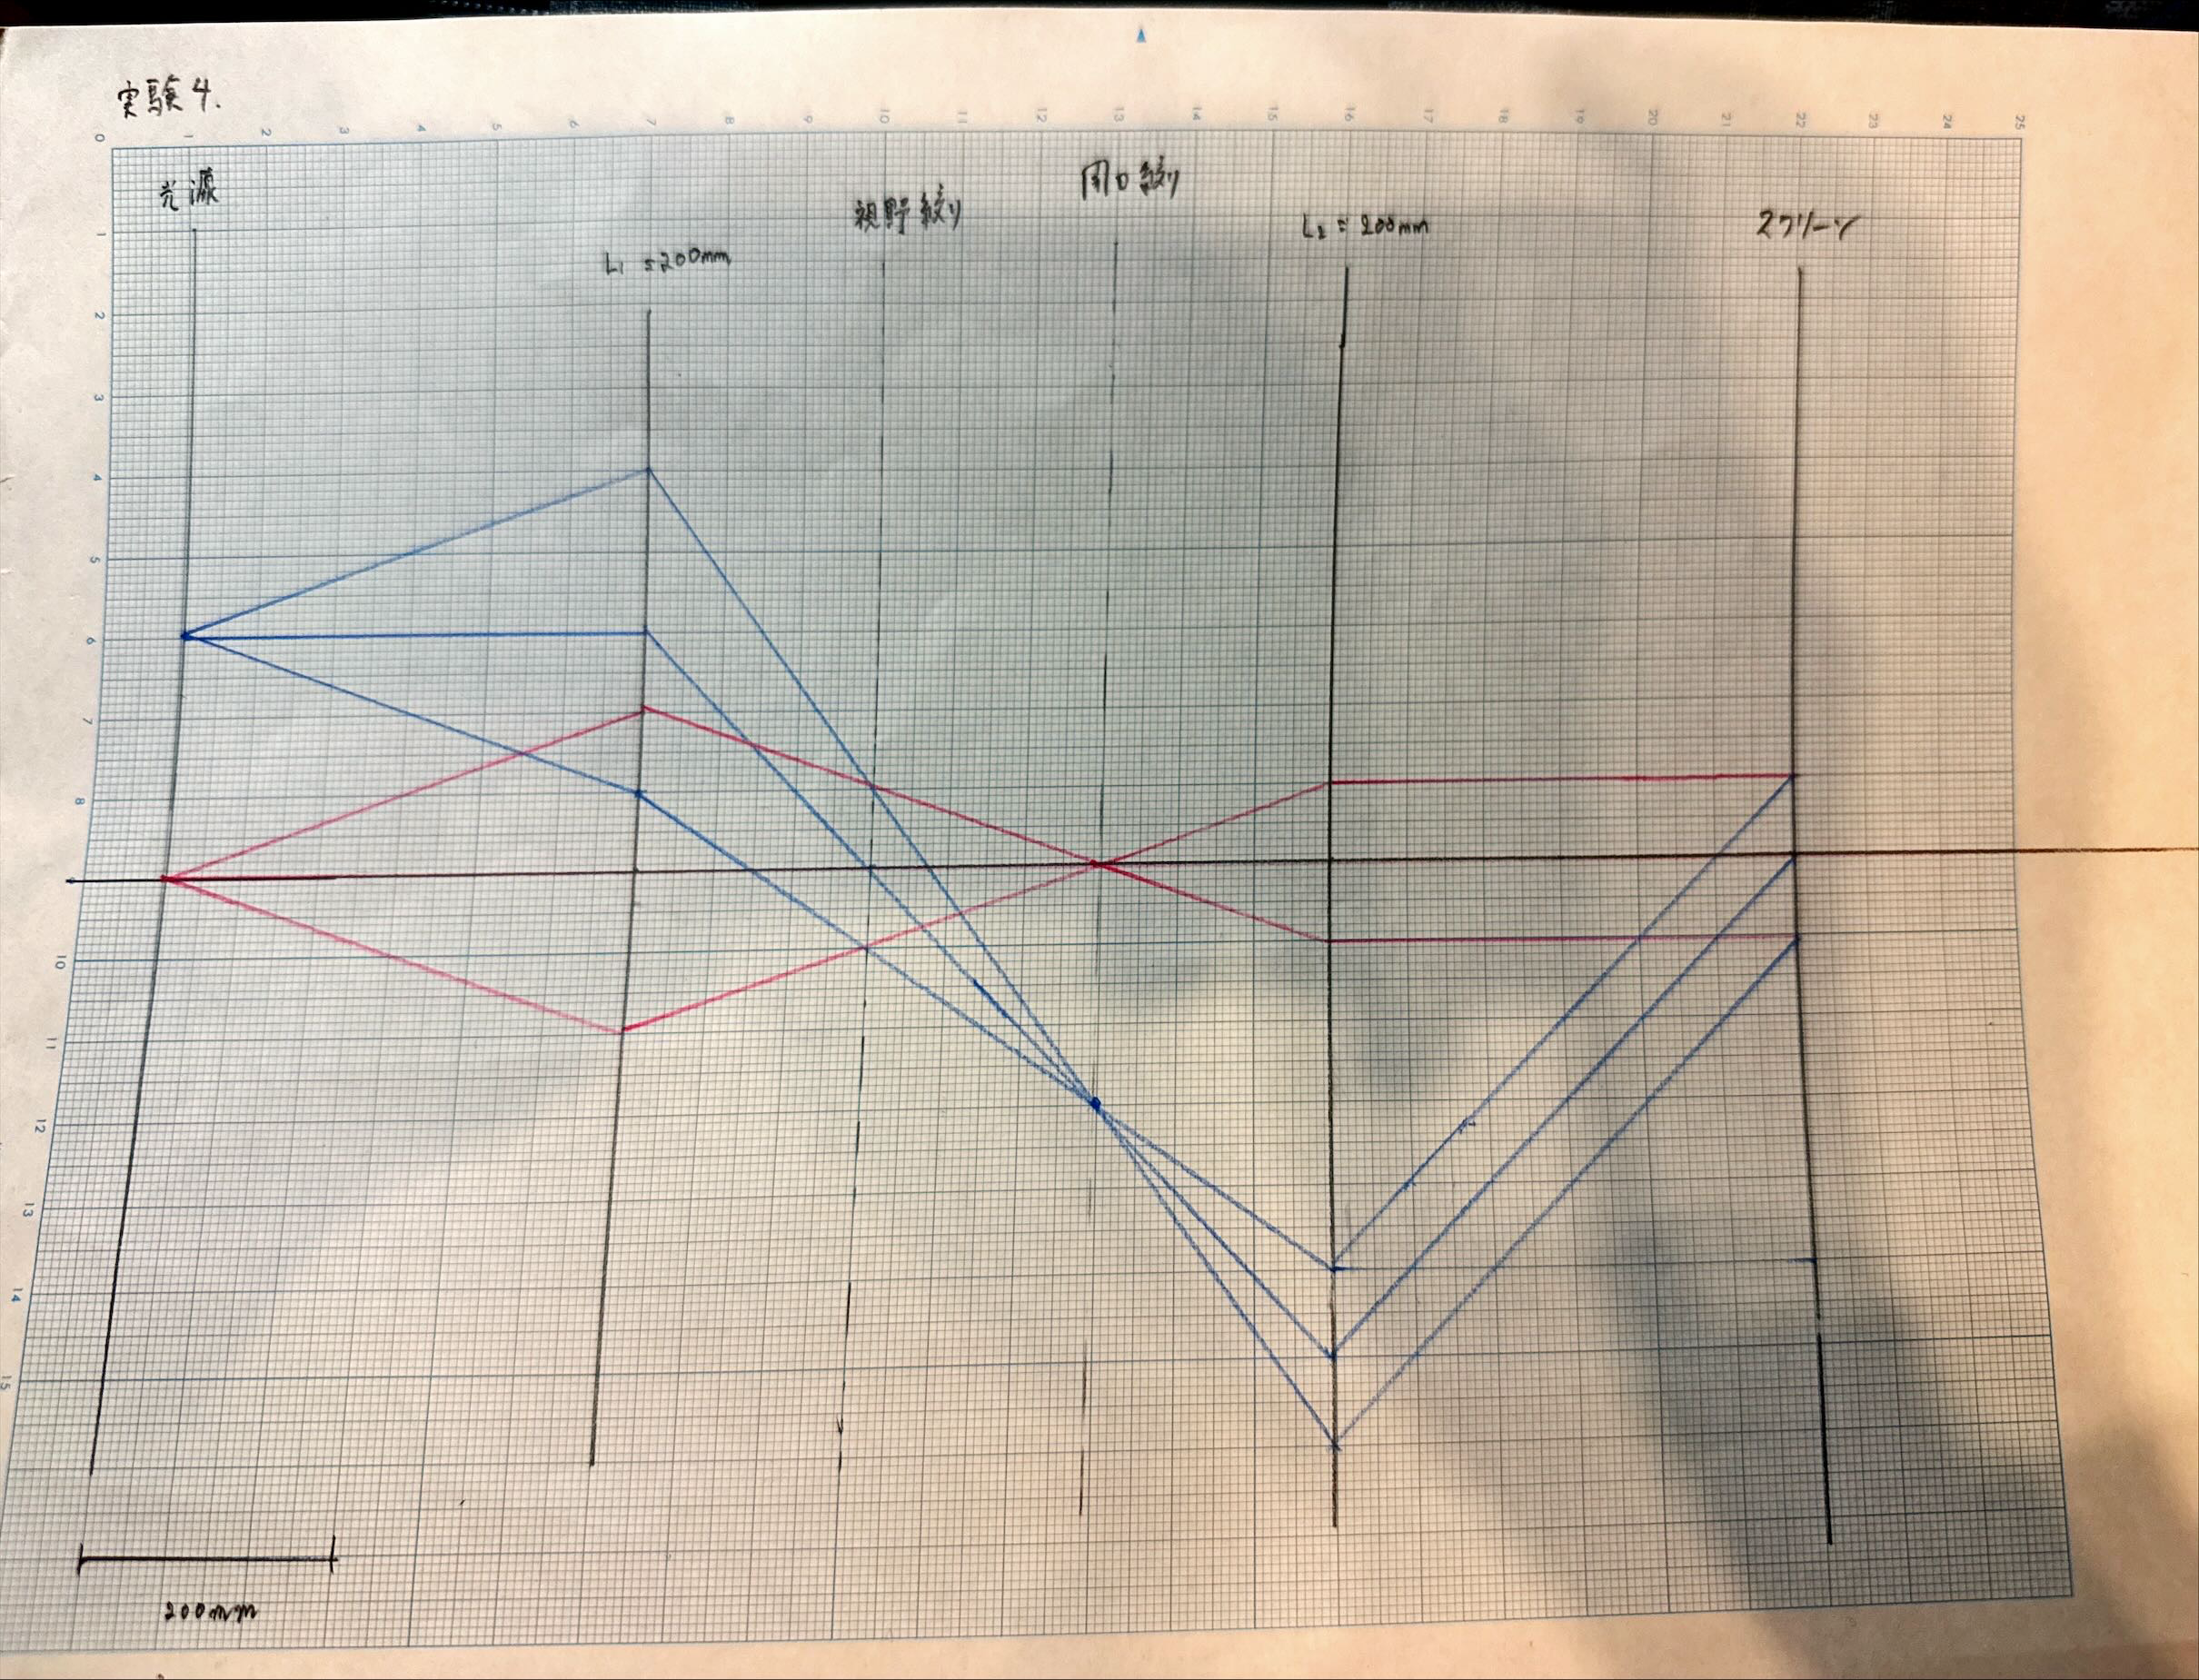
\includegraphics[width=0.98\linewidth]{./figure/4_sakuzu.png}
  \caption{実験4で作成したケーラー照明の作図。視野絞りが試料面に結像し、光源像が開口絞り面に結像することがわかる。}
  \label{fig:kohler_sakuzu}
\end{figure}


\subsection*{\underline{結果}}
視野絞りが試料面に、光源像が開口絞り面にそれぞれ結像していることを確認し、
両絞りを独立に調整することで視野の一様性と照明の角度分布(NA)を独立に制御できることが確認された。

  \subsection*{\underline{考察}}
  \subsection*{レポートのための課題4}

  \begin{enumerate}
    \item 視野絞り:コンデンサーレンズに関して、スクリーンと共役な位置にあるから。\\
開口絞り:集光レンズに関して、光源と共役な位置にあるから。
    \item 図\ref{fig:kohler_sakuzu}にあるように、800mmの位置はコンデンサーレンズの焦点であるが、同時に光源の集光レンズに関する共役点でもある。
    これによって、開口絞りの位置に光源があるのと同様の状態が実現しており、一様な照明が実現する。
  \end{enumerate}

\section*{実験5. 顕微鏡の組立}
\subsection*{\underline{目的}}
実験4で構成したケーラー照明系を照明系として用い、対物レンズ($f=70\,\mathrm{mm}$)と結像レンズ($f=500\,\mathrm{mm}$)からなる観察系を組み上げて、簡易顕微鏡を構成することを目的とする。
その上で、格子縞試料($20\,\mu\mathrm{m}$、$100\,\mu\mathrm{m}$間隔)の像がカメラ上に結像することを確認し、必要な焦点調整と光軸調整を行う。
さらに、視野絞り直後に650\,nmフィルタを挿入した際の像の変化を観察し、顕微鏡光学系の共役関係と調整手順を理解する。



\section*{実験の感想}
\subsubsection*{Day1}
目に見えるのが嬉しい。
\end{document}

% 実験4までDONE
% NA: 実験5。目的の文章だいぶ怪しい。
